\section{OAL 框架与文献映射}\label{sec:oal}

OAL 对\emph{判断什么}、\emph{寻求哪种主张}以及\emph{何时需要该主张}进行分类。某个机制可以支持多个单元格；某些组合可能不适用于某项任务。主张之间的依赖关系另行表示，因此分类不意味着证据相互独立。

\subsection{对象、保障层与生命周期}

\emph{实体}是可问责的主体：组织、操作人员、服务，或具有委托权限的自主代理。\emph{平台/设备}是执行功能的端点，包括无人平台、网关、传感器和承载的计算实例。当航行器行使委托权限时，可将其视为实体；测量其固件状态时，则将其视为平台。\emph{链路/路径}包括端到端路由上的物理介质、中间节点、安全关联和变化的质量。\emph{数据产品}是具有明确版本标识的观测、轨迹、地图、模型、命令、策略或审计记录。更正与转换会产生新的版本标识符。表~\ref{tab:objects} 汇总各类对象的证据和依赖问题。

\begin{table}[H]\small
\caption{OAL 对象及针对具体主张的证据。}\label{tab:objects}
\begin{tabularx}{\textwidth}{@{}P{26mm}YY@{}}\toprule
\textbf{对象} & \textbf{证据} & \textbf{依赖问题}\\\midrule
实体（E） & 凭证、角色、委托、可问责的行为 & 谁在行动，依据什么权限？\\
平台（P） & 启动/运行时测量、配置、自检、能源 & 哪个端点在执行，其测得状态如何？\\
链路/路径（L） & 认证、路由、时延、丢失、托管及介质状态 & 路径上具备什么保护与时效性？\\
数据产品（D） & 签名、内容标识、时间、谱系、不确定性、残差 & 这是哪个版本，什么证据支持其预期用途？\\\bottomrule
\end{tabularx}\end{table}

保障轴包括 O（观测有效性）、C（承诺与溯源完整性）、G（账本与治理一致性）和 M（任务使用适合性）。O 使用物理边界、校准、诊断和交叉佐证。C 通过签名与溯源绑定生产者、版本和转换断言。G 处理共同授权的成员资格、顺序、策略和恢复状态。M 应用目的、时效性、后果、不确定性和权限要求。当不需要共享状态服务时，账本特有主张不适用；等价的治理主张可以由其他服务满足。

策略、模型和参考值是带版本的数据产品；其部署实例位于平台上，其批准权限属于实体。这种处理使保障基础设施与任务观测接受相同的分析。单元格规范首先确定对象/版本及所需属性，再给出支撑证据和有效时间区间。它还指明接受规则、责任方，以及证据缺失时的响应。表~\ref{tab:lifecycle} 汇总生命周期阶段与状态转换。

\begin{table}[H]\small
\caption{生命周期阶段及相关状态转换。}\label{tab:lifecycle}
\begin{tabularx}{\textwidth}{@{}P{30mm}YY@{}}\toprule
\textbf{阶段} & \textbf{所需保障} & \textbf{保留状态示例}\\\midrule
准入（A） & 主体经过授权，端点符合接受要求 & 角色、委托、证明参考\\
感知（S） & 时间、位置和观测可信 & 产品标识、质量和采集承诺\\
传输（T） & 内容受保护，路径满足要求 & 中继/托管事件和批次根\\
融合/共享（F） & 输入、转换和访问均有明确标识 & 谱系、模型和策略版本\\
决策/行动（D） & 当前适合所指定的后果 & 决策依据和责任主体\\
恢复/审计（R） & 明确失效范围并恢复权限 & 撤销、争议和协调后的历史\\\bottomrule
\end{tabularx}\end{table}

\subsection{编码样本中观测到的覆盖情况}\label{sec:coverage}

图~\ref{fig:oal} 映射了来自 39 项研究的 89 项主张。96 个可能的单元格中，有 25 个包含已编码主张。处理/融合阶段的数据治理（D/G/F）是最大的单元格，包含 16 项研究。71 个零值单元格在本样本中没有编码主张；其适用性取决于任务。单元格计数也存在重叠：一项研究可以同时保护记录、复制记录，并支持其后续审计。

分层结果呈现不同重点。在 19 项面向 UAV、海事 AIS 或水下应用的研究中，准入阶段的实体治理（E/G/A）是最大的单元格，包含 6 项研究。在 20 项可迁移研究中，D/G/F 以 11 项居首。因此，总体集中趋势部分源于溯源与共享状态基础设施的纳入。每项主张均已对照其支撑段落与评估环境进行核查。

\subsection{比较如何改变设计审查}\label{sec:comparative}

OAL 各轴将某种机制提供的证据，与其下游使用者的要求区分开。表~\ref{tab:interfaces} 比较了应用标签或信任词汇相似、但支持不同依赖决策的机制。表~\ref{tab:sensitivity} 报告对领域选择与编码选择的敏感性。

\begin{table}[H]\footnotesize
\caption{OAL 比较揭示的主张边界。最后一列说明组合这些机制时的附加要求。}\label{tab:interfaces}
\begin{tabularx}{\textwidth}{LLL}\toprule
\textbf{机制比较} & \textbf{提供的证据} & \textbf{对机制组合的影响}\\\midrule
AIS 保护与接收机账本（S27--S29） & 发送者/消息保护（E/C/T、D/C/T）与接收机提交的历史（F/R 阶段的 D/C 和 D/G）具有不同信任边界 & 保留与原始发送者的绑定；使用位置执行行动前，要求观测评估和时效性证据\\
视觉与多观察者佐证（S24--S25、S39） & 在纹理、几何和观察者假设下，轨迹一致性或报告一致性支持感知/融合阶段的 D/O & 将这些假设随结果保留；经过认证的一致意见本身不能排除相关误差\\
证明与伙伴选择（S12、S14、S26、S34） & 测得的端点/模型完整性不同于任务特定的卸载或更新适用性 & 同时检查执行状态与任务证据；凭证和信任分数都不能替代对方所支持的主张\\
UAV 信任与路由（S30--S31、S39） & 行为变化可以触发排除或路径调整（E/M、L/M 和 E/G） & 复用这些连续性机制，再规定断连期间的权限与依赖产品处理\\
复制状态协议（S35--S38） & 相似的 D/G/F 或 D/G/R 单元格仍保留不同故障模型、同步假设和已测试恢复路径 & 比较时延前先选择假设；仅恢复复制日志并不会使派生任务产品失效\\\bottomrule
\end{tabularx}\end{table}

\begin{figure}[!htbp]\centering
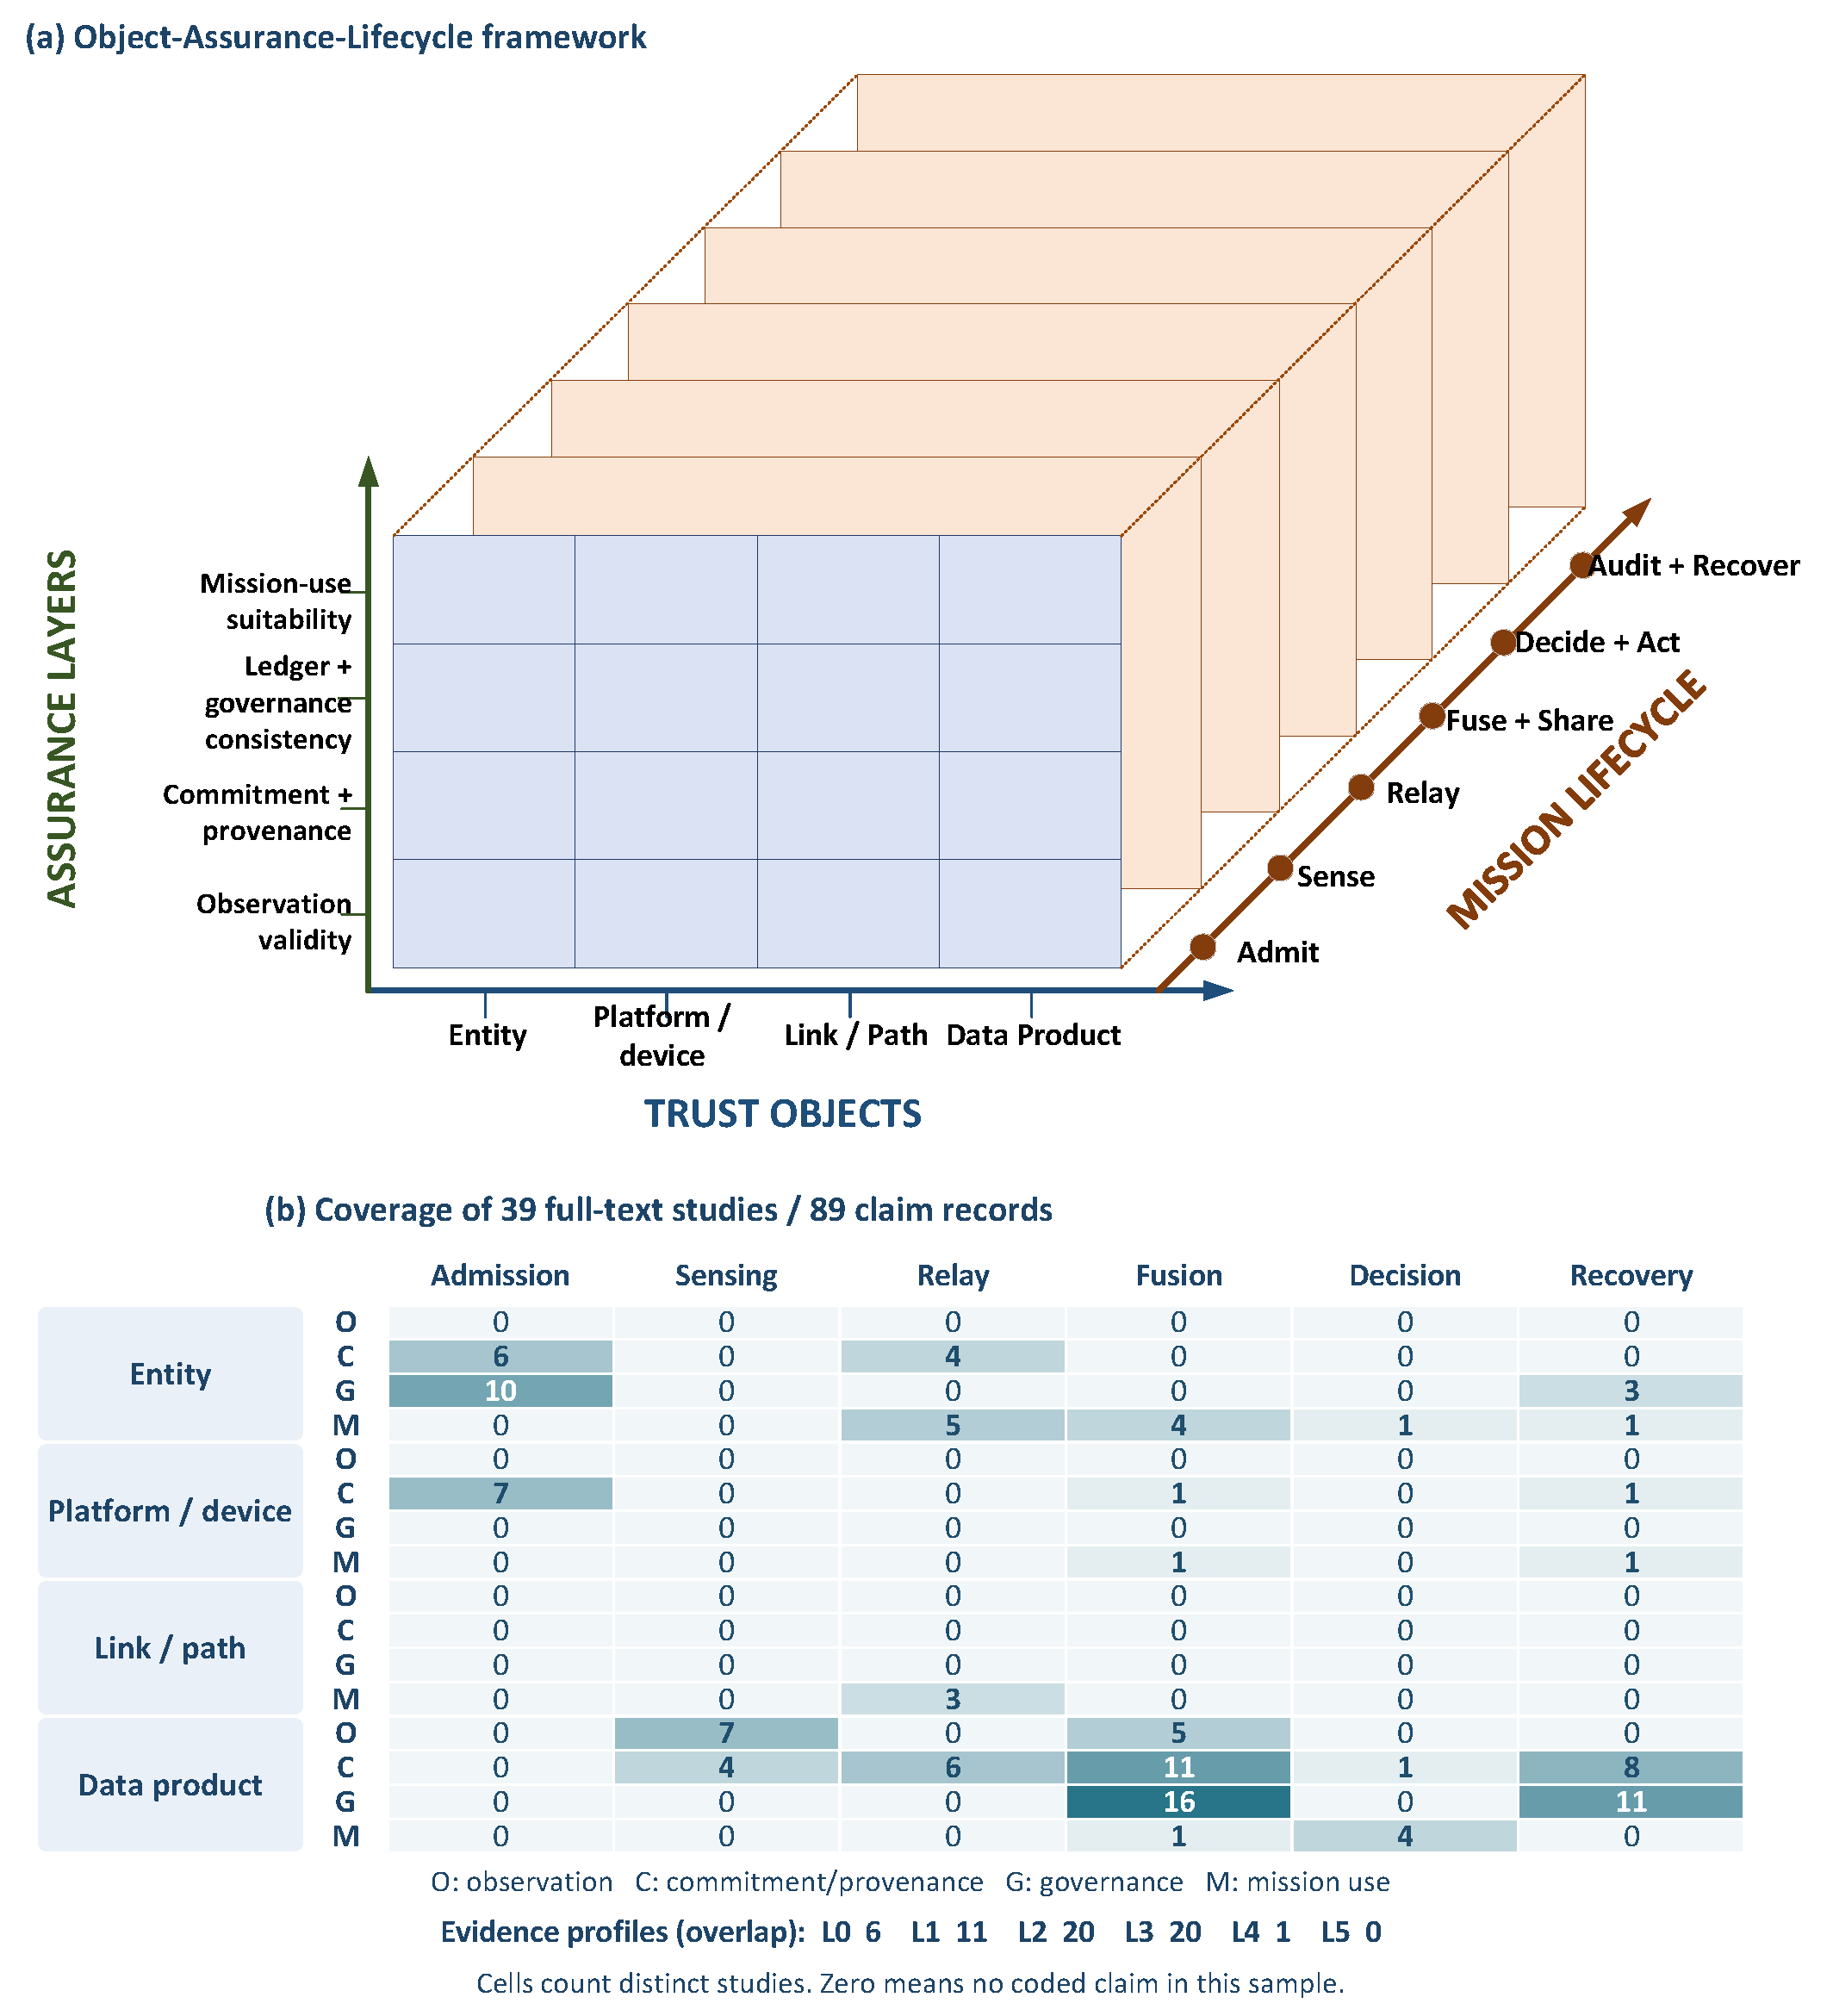
\includegraphics[width=.91\textwidth,height=.73\textheight,keepaspectratio]{figures/figure-03-oal-framework.pdf}
\caption{OAL 框架与 39 项全文机制研究的映射。（\textbf{a}）对象、保障和生命周期维度。（\textbf{b}）由 89 条限定范围的主张记录计算得到的各确切单元格中的不同研究数。证据类型计数存在重叠。零表示没有已编码主张，并不据此确定适用性或整个研究领域的空白。表~\ref{tab:sensitivity} 区分领域效应与纳入效应。}\label{fig:oal}
\end{figure}

\begin{table}[H]\small
\caption{覆盖图谱的敏感性。被覆盖单元格数是描述性计数，不是完整性评分。D/G/F 表示融合阶段的数据治理；E/G/A 表示准入阶段的实体治理。}\label{tab:sensitivity}
\begin{tabularx}{\textwidth}{@{}YrrP{32mm}@{}}\toprule
\textbf{纳入研究/编码变体} & \textbf{研究数} & \textbf{单元格数} & \textbf{最大单元格（计数）}\\\midrule
全部研究 & 39 & 25 & D/G/F（16）\\
直接领域层 & 19 & 18 & E/G/A（6）\\
可迁移层 & 20 & 20 & D/G/F（11）\\
去除四项通用共识比较研究 & 35 & 25 & D/G/F（12）\\
去除仅有概念证据的研究 & 35 & 22 & D/G/F（15）\\
直接领域层去除代理数据研究 & 18 & 17 & E/G/A（6）\\
准入身份仅归属于实体 & 39 & 25 & D/G/F（16）\\
逐一剔除研究（39 次运行） & 38 & 23--25 & D/G/F（15--16）\\\bottomrule
\end{tabularx}\end{table}

AIS 比较展示了一次保障交接。海事监测原型记录经过授权的接收机提交的观测\citep{maritime2022monitoring}；pAIS 和 SecAIS 则考察 AIS 消息保护\citep{kessler2020protected,goudossis2022secais}。pAIS 演示使用较弱的演示参数，SecAIS 则通过仿真 AIS 设备实现所选模式。它们的 L3 类型说明存在软件实现，并不意味着安全强度相同或已经完成无线实传验证。依赖这些信息的导航服务仍需获得有关所报告位置的证据。视觉里程计交叉检查提供了这样一种机制，其评估基于记录数据，并存在低纹理水面或夜间条件下的局限\citep{varshosaz2019spoofing}。多 UAV 交叉佐证在对观察者和恶意参与者作出假设的条件下，提供另一种机制\citep{garcamagario2019security,barka2022towards}。OAL 揭示了这样一个环节：如果接受规则规定不充分，带有签名、存储一致但内容错误的位置仍可能通过检查。

UAV 信任与路由研究提供了保持连续性的先例。分层无人机信任和区块链辅助路由，会随行为变化更新声誉并限制协作\citep{hierarchical2023trust,yang2023trusted}。Yang 等报告了一项限定范围的实验，涉及八个实体 UAV 节点、定时恶意转发和链路中断。这支持协作/路径调整主张（L3/L4）；其更大规模的共识基准测试使用独立容器环境。这些机制已经将行为观测与持续使用相联系。联盟场景新增的问题是：处于分区中的参与方如何解释权限变化，并将失效处理传播到依赖产品。第~\ref{sec:trace} 节进一步展开这一问题。

任务适用性同样具有特定范围。COMITMENT 将伙伴历史与工作负载/容量标准结合，用于雾计算卸载\citep{alkhafajiy2020comitment}。水下签密研究在桌面环境中评估密码运算，信任/能量路由则使用仿真\citep{zhang2026underwater,eetauv2025trust}。TAFL-UWSN 对联邦参与方和更新进行筛选，但其详细评估使用陆地 UNSW-NB15 数据\citep{tafl2026underwater}。这些结果分别支持不同的承诺或处理决策；将其迁移到声学任务，还需要信道、能耗和数据分布证据。

最后，落入同一单元格并不意味着机制可以互换。Raft 与拜占庭协议的故障假设不同\citep{raft2014,pbft1999,hotstuff2019,narwhal2022}。最初的 PBFT 原型没有实现视图变更或重传，因此其正常运行主张获得 L1/L3，而恢复主张获得 L1。这种主张层面的区分，避免把原型标签扩展到未经测试的路径。在整个样本中，没有提取出的主张证明：一个集成的空中-水面-水下任务，已经同时验证权限连续性、观测评估和依赖产品恢复。

\subsection{对选择与编码的敏感性}\label{sec:sensitivity}

表~\ref{tab:sensitivity} 汇总纳入和编码选择如何改变覆盖图谱。去除四篇通用共识论文后，25 个被覆盖单元格全部保留，领先单元格不变，其研究数降为 12。去除四项仅有概念证据的研究后，被覆盖单元格减少到 22。因此，基础设施比较研究增加了计数，而部分覆盖依赖概念性机制。去除使用陆地代理数据的研究后，直接领域层仍以准入治理为中心。

将 S01--S03 的平台身份编码行重新归为实体身份，会改变个别单元格计数，但不会改变被覆盖单元格数或领先单元格。每次逐一剔除分析都保留 D/G/F 为最大单元格，总体被覆盖单元格数为 23--25。L4 计数取决于 S31：若保守地将其限定范围的实体节点实验归为试验台，则 L4 消失，热图不变。领先单元格对移除单项研究保持稳定，而领域分层与主张层面的比较揭示了不同的组合要求。
